\setAuthor{Mihkel Pajusalu}
\setRound{piirkonnavoor}
\setYear{2012}
\setNumber{G 8}
\setDifficulty{7}
\setTopic{Elektriahelad}

\prob{Raudtee}
\begin{wrapfigure}{r}{18mm}%
\vspace{-15pt}
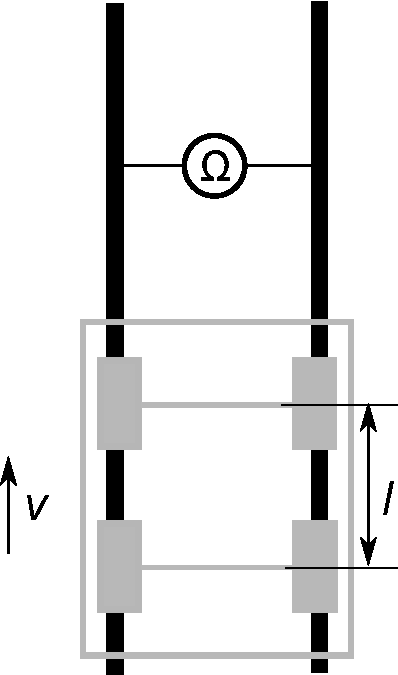
\includegraphics[width=\linewidth]{2012-v2g-08-rong}%
\end{wrapfigure}
Mõõdame raudteel elektritakistust kahe kõrvutise rööpa vahel nii, nagu joonisel.
Rööbastel sõidab vagun kiirusega $v$. Olgu vagunil kaks rattapaari,
mille vahekaugus on $l$. Joonistage graafik takistuse muutumisest ajas alates
hetkest, kui vaguni esimene rattapaar on mõõtepunkti ees sellest kaugusel $l/2$, kuni
ajani, kui tagumine rattapaar on mõõtepunkti taga sellest kaugusel $l/2$. Mõlema rattapaari
takistuseks olgu $r$ ja rööpa takistus pikkusühiku kohta $\rho$.

\hint
Ülesandes peab käsitlema kahte juhtu: a) kui mõõtepunkt ei asu vaguni rataste vahel ja b) kui mõõtepunkt asub vaguni rataste vahel. Mõlemal juhul käitub tekkiv elektriskeem isemoodi.

\solu
\begin{wrapfigure}{r}{50mm}
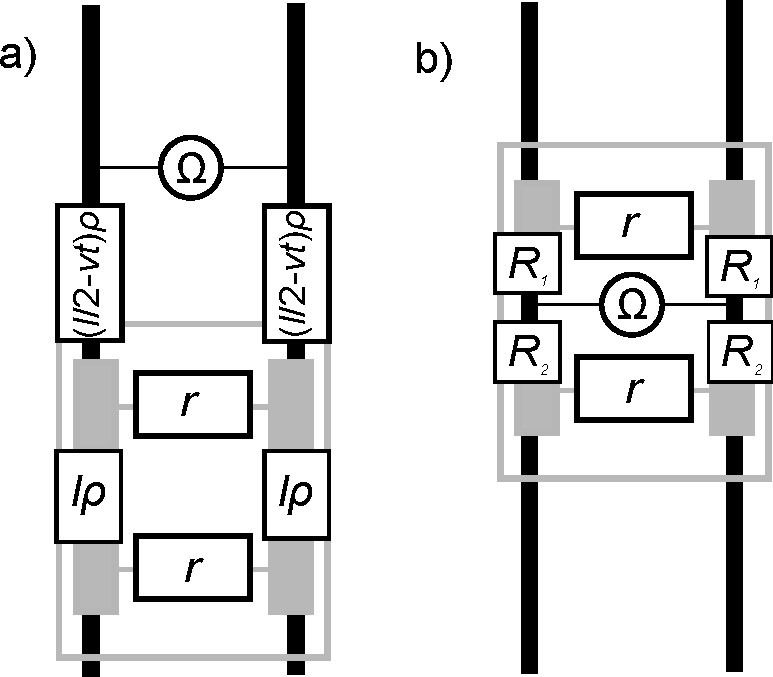
\includegraphics[width=\linewidth]{2012-v2g-08-rong_lahendus}
\end{wrapfigure}
Ülesandes peab käsitlema kahte juhtu: a) kui mõõtepunkt ei asu vaguni rataste vahel ja b) kui mõõtepunkt asub vaguni rataste vahel. On ka näha, et ülesanne on sümmeetriline mõõtepunkti suhtes, st takistuse käitumine enne seda, kui vaguni keskpunkt möödub mõõtepunktist ja pärast seda, on üksteise peegelpildid.

Vaatleme alguses juhtu a). On näha, et sellel juhul on vagunil fikseeritud takistus, millele liitub vaguni ja mõõtepunkti vahele jäävate rööbaste takistus.
\[
R=2(l/2-vt)\rho+\frac{1}{\frac{1}{r}+\frac{1}{r+2l\rho}}.
\]

Seejärel vaatleme juhtu b). Sellel juhul moodustub takistus kahest rööpühenduses olevast osast, mille takistus muutub vaguni liikumise käigus. $R_1=(l-vt')\rho$ ja $R_2=vt'\rho$, kus $t'=t-s/v$ on aeg, mis on möödunud hetkest, kui esimene rattapaar möödus mõõtepunktist. Seega saab takistuse käitumise leida valemist:
\[
R=\frac{1}{\frac{1}{r+2R_1}+\frac{1}{r+2R_2}}=\frac{1}{\frac{1}{r+2(l-vt')\rho}+\frac{1}{r+2vt'\rho}}.
\]

Tulemuseks on graafik:

\begin{center}
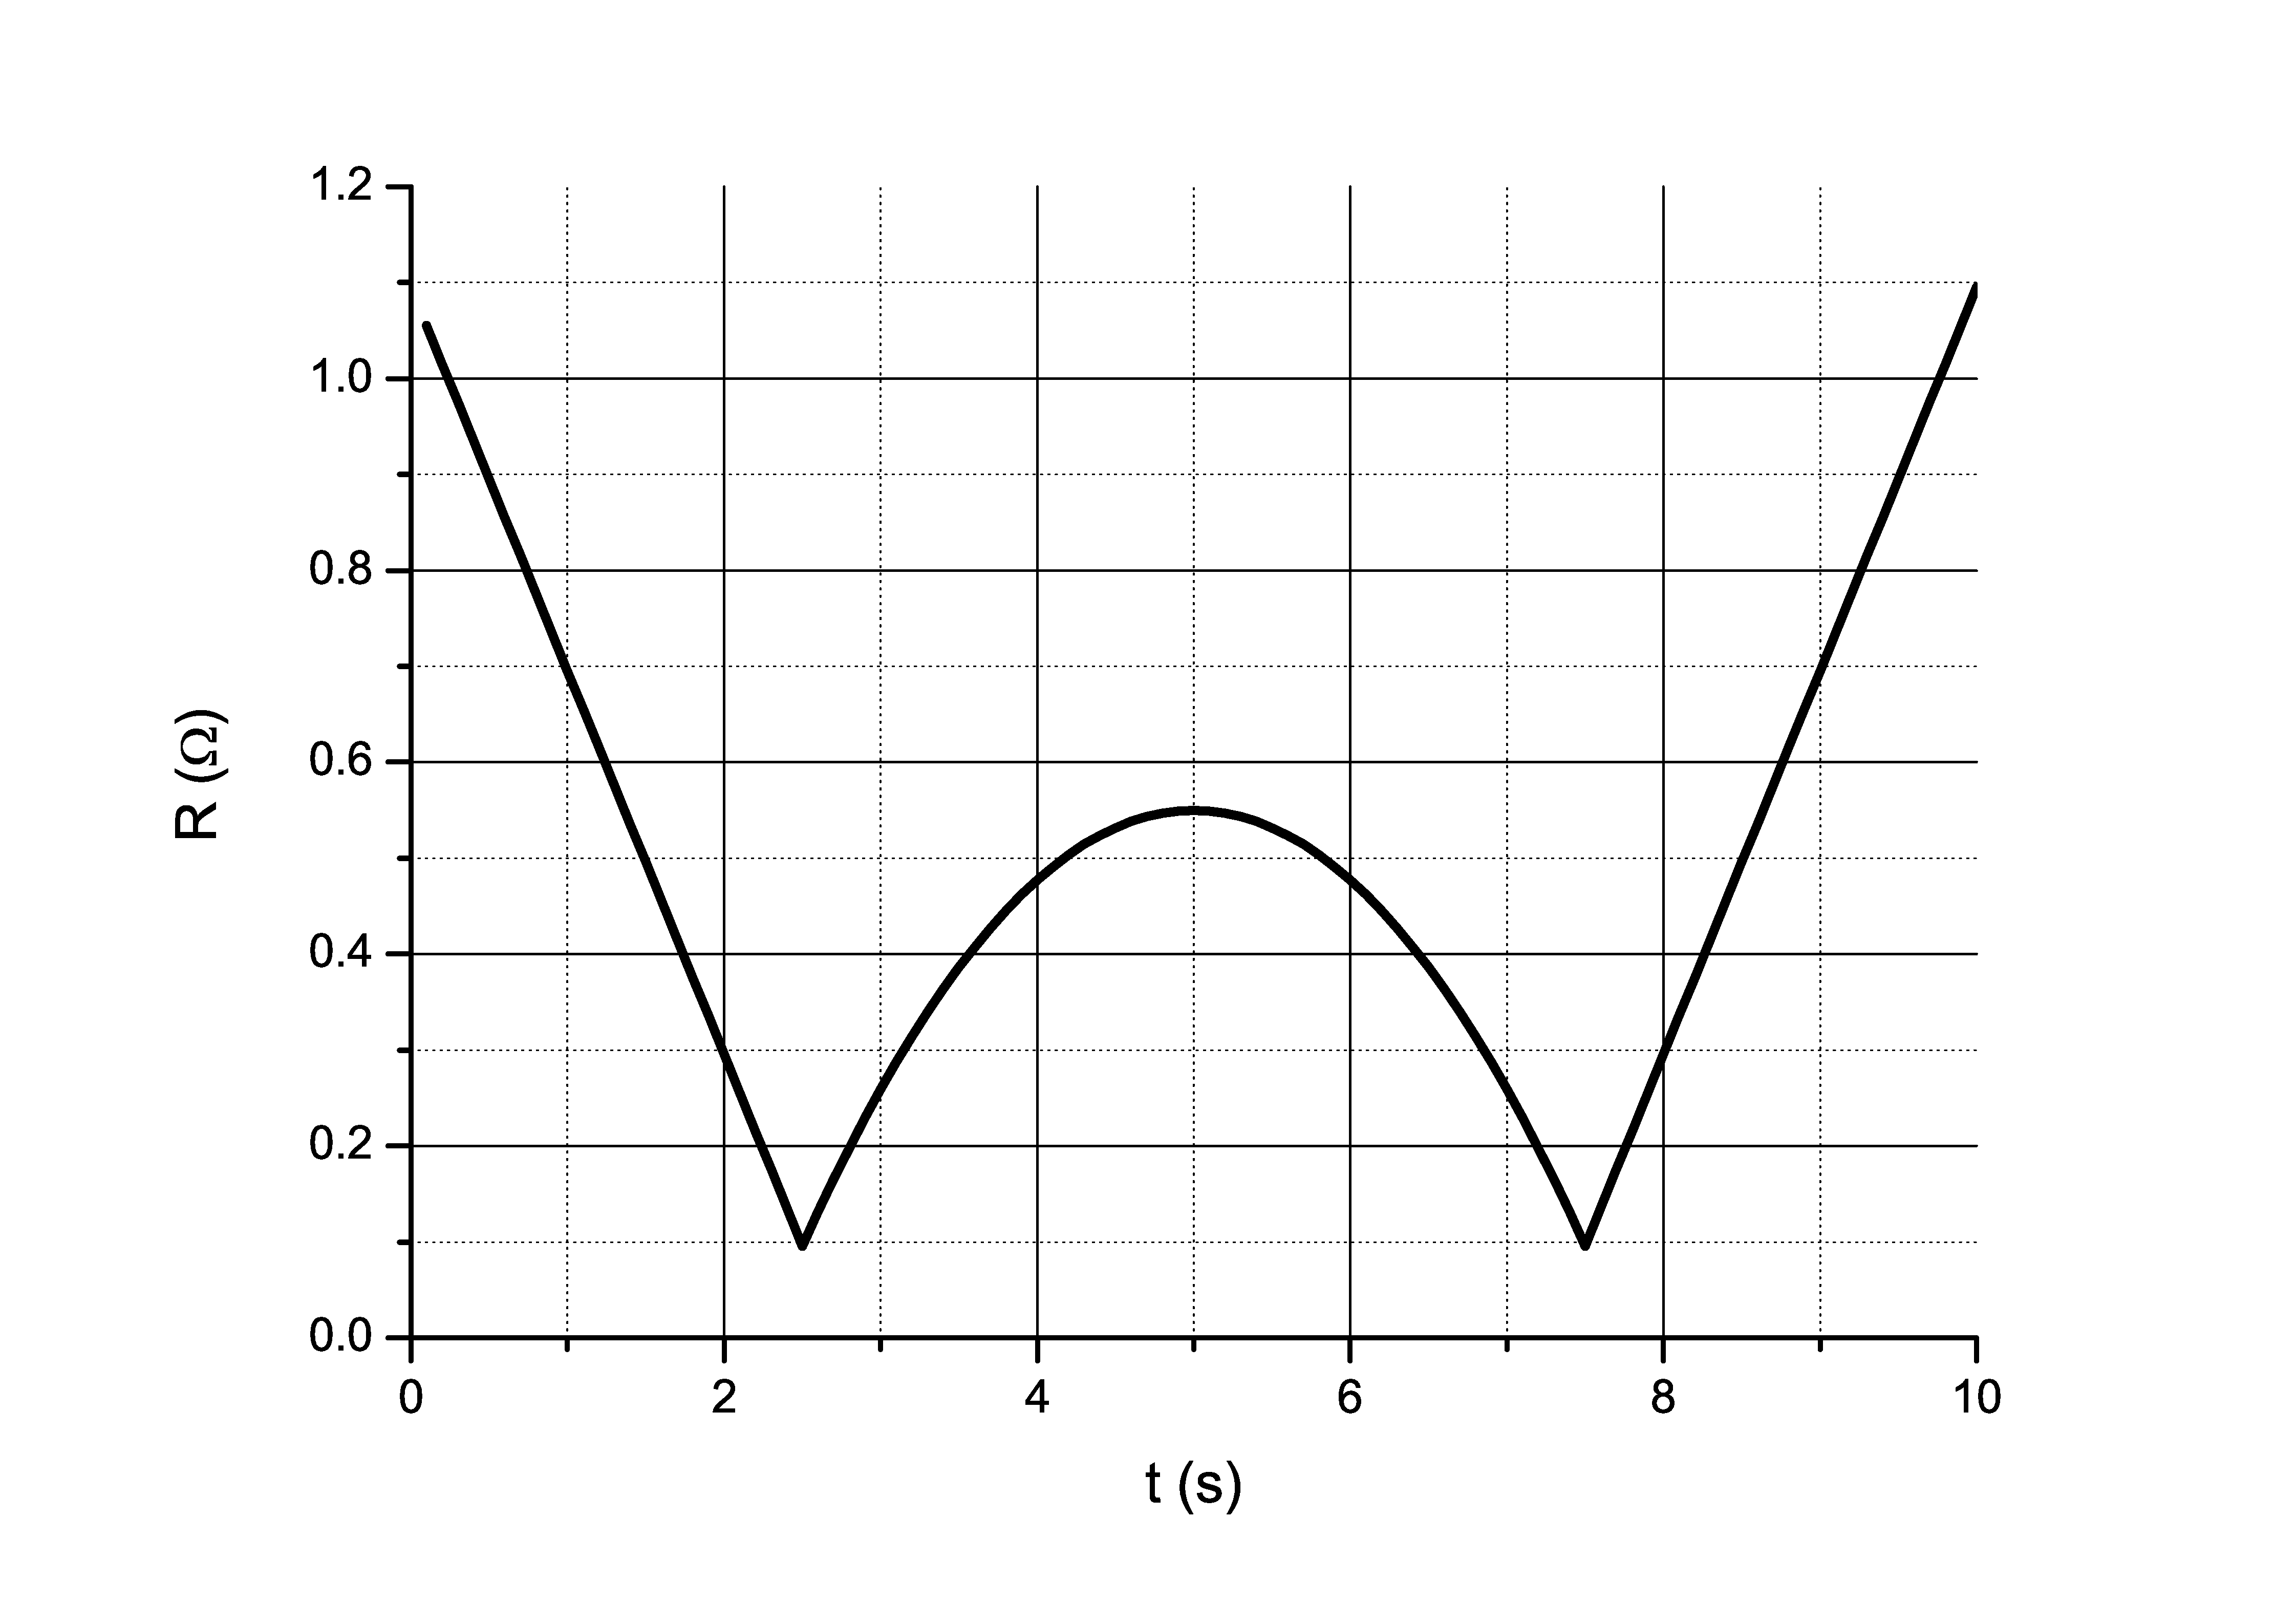
\includegraphics[width=300pt]{2012-v2g-08-rong_graafik}
\end{center}

\probeng{Railway}
\begin{wrapfigure}{r}{18mm}%
\vspace{-15pt}
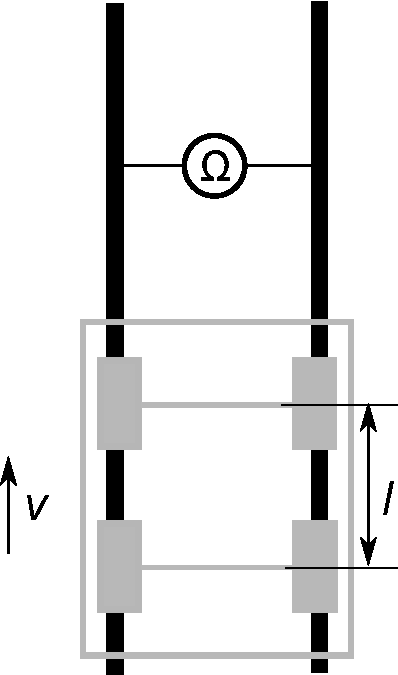
\includegraphics[width=\linewidth]{2012-v2g-08-rong}%
\end{wrapfigure}
Let us measure the electrical resistance between two rails on a railway, like in the drawing. A wagon of speed $v$ drives on the railway. The wagon has two pairs of wheels, one pair is at a distance $l$ from the other. Draw a plot of resistance versus time from the moment when the wagon’s first pair of wheels is at the front of the measuring point at a distance $l/2$ to the moment when the wagon’s rear wheels are behind the measuring point at the distance $l/2$.  Let the resistance of both pairs of the wheels be $r$ and a rail’s resistance per one unit of length $\rho$.

\hinteng
Two cases must be dealt with in the problem: a) if the measuring point is not located between the wagon's wheels and b) if the measuring point is located between the wagon's wheels. For either case the electric circuit created will act differently.

\solueng
\begin{wrapfigure}{r}{50mm}
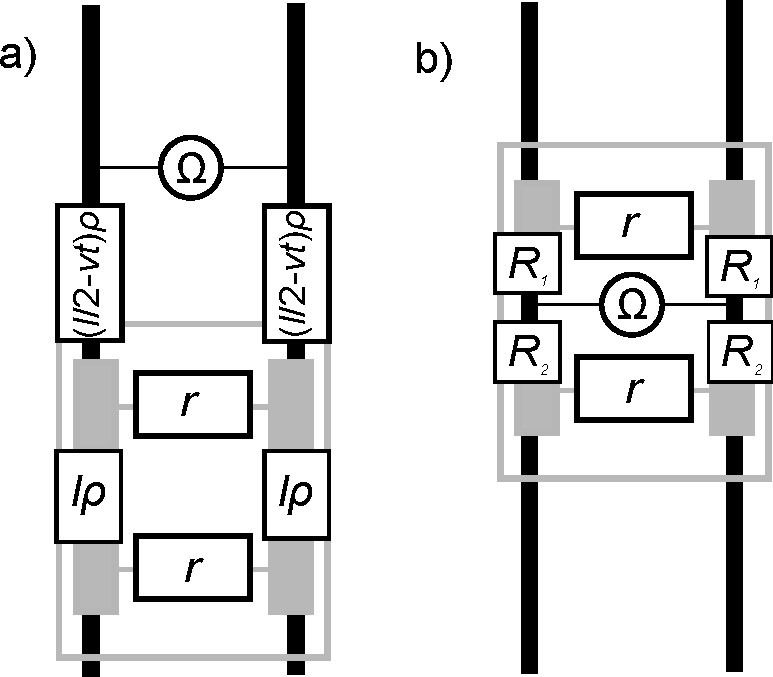
\includegraphics[width=\linewidth]{2012-v2g-08-rong_lahendus}
\end{wrapfigure}
Two cases must be observed in the problem: a) if the measuring point is not located between the wheels of the wagon and b) if the measuring point is located between the wheels of the wagon. It is also clear that the problem is symmetrical with respect to the measuring point meaning that the behavior of the resistor before when the wagon’s center passes the measuring point and after it are each other’s reflections.\\
First let us observe the case a). It can be seen that in this case the wagon has a fixed resistance which is added with the resistance of the rails that stay between the wagon and the measuring point. 
\[
R=2(l/2-vt)\rho+\frac{1}{\frac{1}{r}+\frac{1}{r+2l\rho}}.
\] 
Next let us observe the case b). In this case the resistance is made of two parts that are connected in parallel. Their resistances change in the course of the wagon’s movement. $R_1=(l-vt')\rho$ and $R_2=vt'\rho$ where $t'=t-s/v$ is the time that has passed from the moment where the first pair of wheels went pass the measuring point. Therefore we can find the behavior of the resistance with the equation:
\[
R=\frac{1}{\frac{1}{r+2R_1}+\frac{1}{r+2R_2}}=\frac{1}{\frac{1}{r+2(l-vt')\rho}+\frac{1}{r+2vt'\rho}}.
\] 
This results in a graph:
\begin{center}
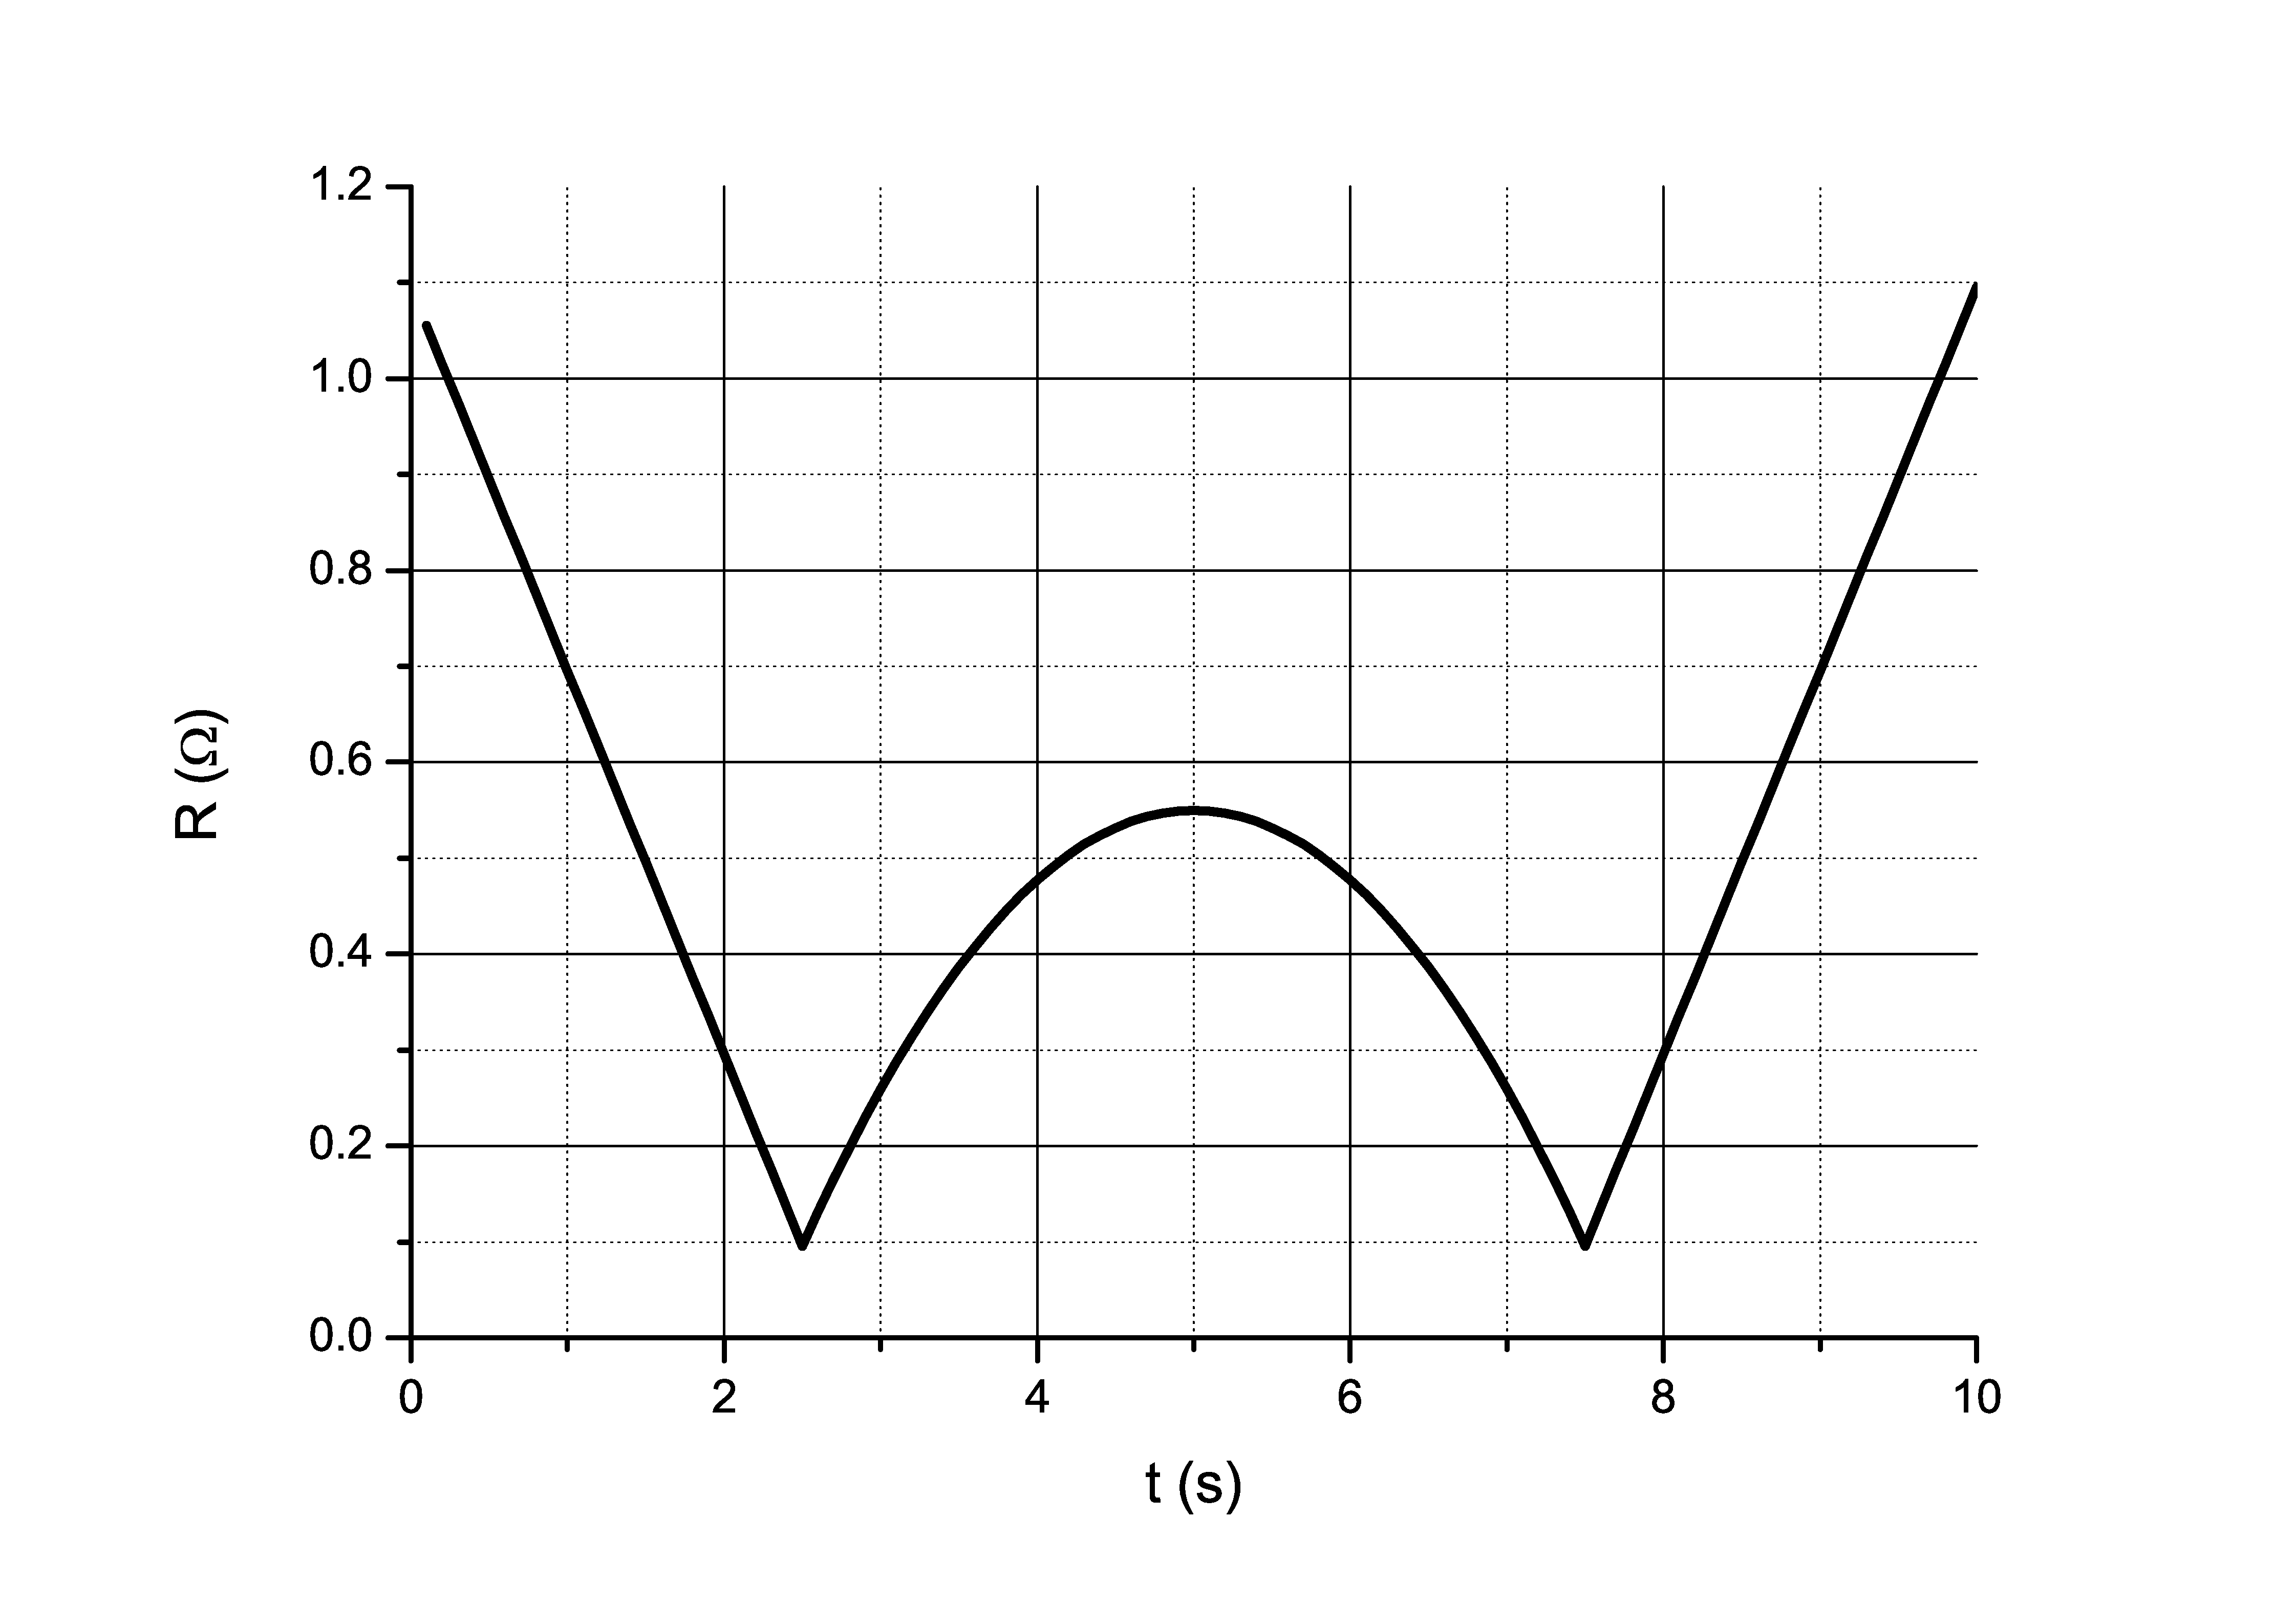
\includegraphics[width=300pt]{2012-v2g-08-rong_graafik}
\end{center}
\probend